
Da bomo lahko asinhrona vezja analizirali in zasnovali potrebujemo povzeti teoretične osnove s katerimi taka vezja modeliramo. Moramo se naučiti kako v takih vezjih signali potujejo in kako dosežemo, da potujejo urejeno. Najosnovnejša metoda ureditve signalov je sinhronizacija.


\section{Sinhronizacija} \label{a}

Sinhronizacija je pojav, kjer dva procesa delita informacije, da delita neko vrednost. V našem primeru je ta vrednost perioda.

\subsection{Osnovna vezja} \label{b}
Najosnovnejše vezje, ki ima periodo je obročni oscilator. Obročni oscilator je narejen iz inverterja, ki povzroči negativno povratno zanko in zakasnilne linije, ki določa periodo oscilatorja.

Začnimo torej z sinhronizacijo dveh obročnih oscilatorjev. Za ta namen potrebujemo posebna logična vrata.

\subsubsection{Muller C element} \label{c}
Muller C element je osnovni element sinhronizacije dveh signalov. Ima dva vhoda, izhod se spremeni, ko sta oba vhoda enaka.

\begin{figure}
	\centering
	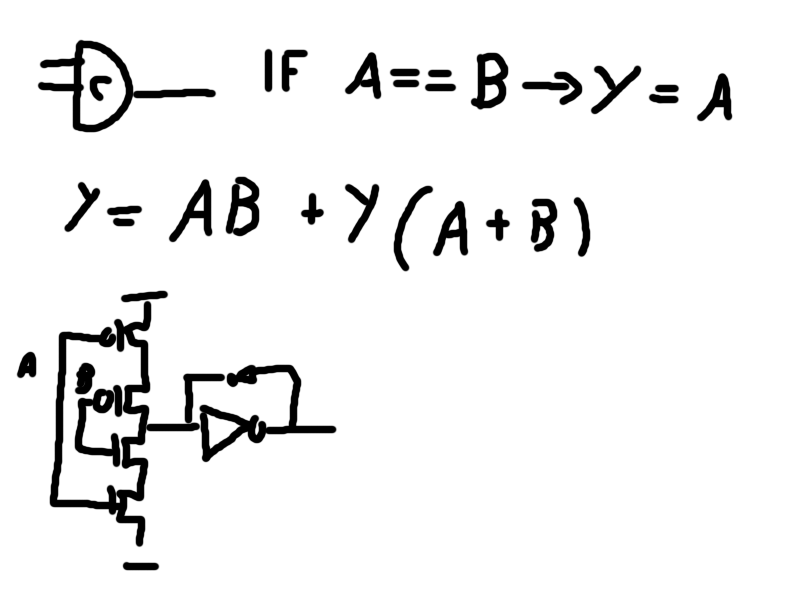
\includegraphics[width=0.7\linewidth]{slike/C_Element}
	\caption{}
	\label{fig:celement}
\end{figure}

Poglejmo si kako tak element sinhronizira dva signala:

\subsubsection{Vzporedna sinhronizacija} \label{c}

Imamo dve povratni zanki, vsaka z različno zakasnitvjo, kateri želimo sinhronizirati.

\begin{figure}
	\centering
	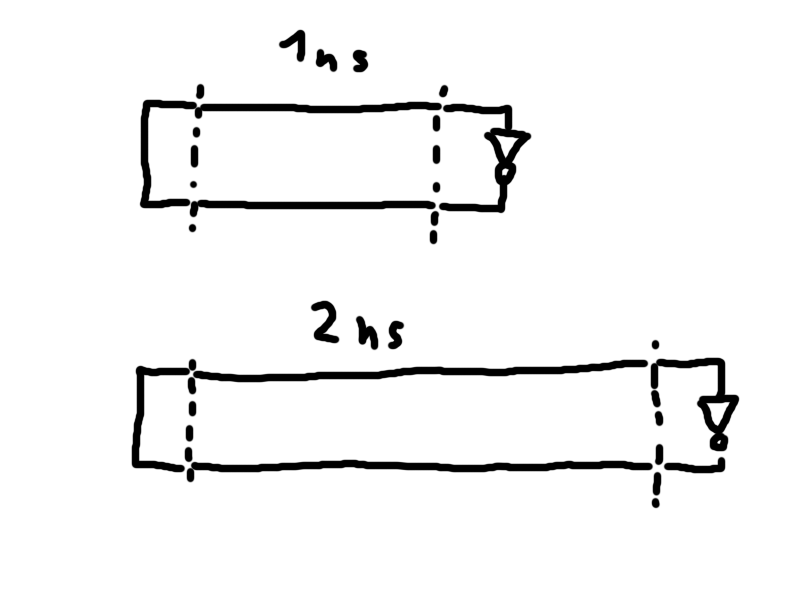
\includegraphics[width=0.7\linewidth]{slike/dly1}
	\caption{}
	\label{fig:celement}
\end{figure}

Če ustvarimo prek C elementa skupno povratno zanko, mora hirejši vedno čakati počasnejšega, torej sta sinhronizirana.

\begin{figure}
	\centering
	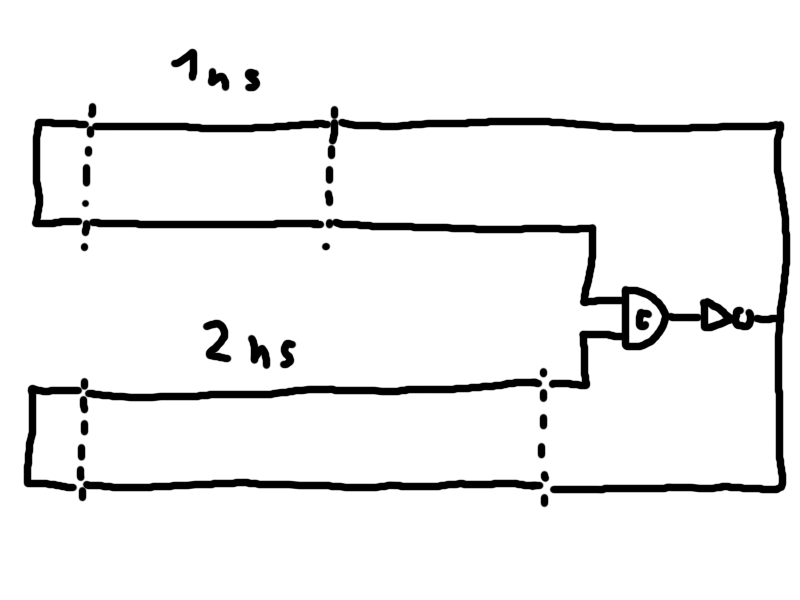
\includegraphics[width=0.7\linewidth]{slike/dly2}
	\caption{}
	\label{fig:celement}
\end{figure}

Trivialno lahko sinhroniziramo poljubno število povratnih zank.

\begin{figure}
	\centering
	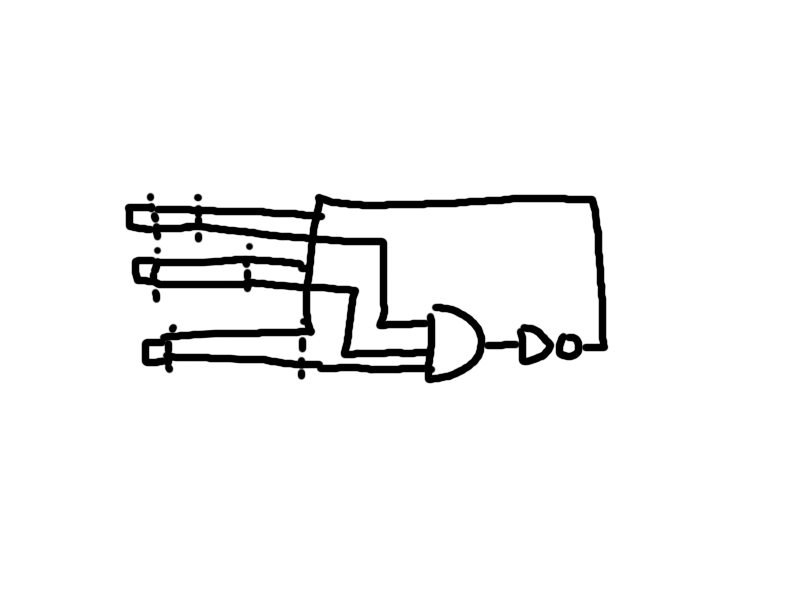
\includegraphics[width=0.7\linewidth]{slike/dly3}
	\caption{}
	\label{fig:celement}
\end{figure}

To lahko razumemo kot vzporedno vezavo oscilatorjev, kjer je skupna perioda, perioda najdaljše povratne zanke. 

\subsubsection{Zaporedna sinhronizacija} \label{c}
Lahko pa vežemo oscilatorje tudi zaporedno na sledeči način:

%Inverter na napacni strani

\begin{figure}
	\centering
	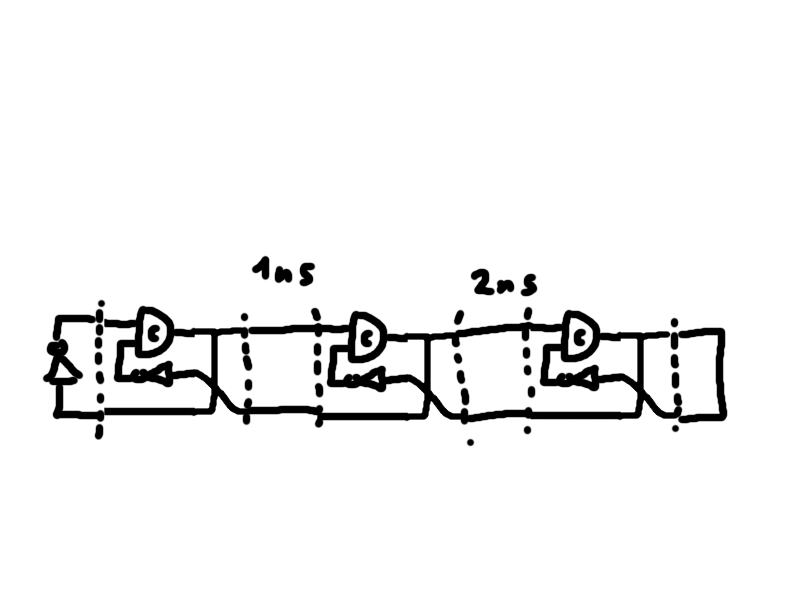
\includegraphics[width=0.7\linewidth]{slike/dly4}
	\caption{}
	\label{fig:celement}
\end{figure}

Tu povratne zanke prepletemo med seboj. Vsako povratno zanko sprožijo njeni sosedje. V tem primeru prva zanka sproži drugo. Ko druga konča ponovno sporži prvo.

Tak vzorec lahko nadaljujemo poljubno dolgo.
\begin{figure}
	\centering
	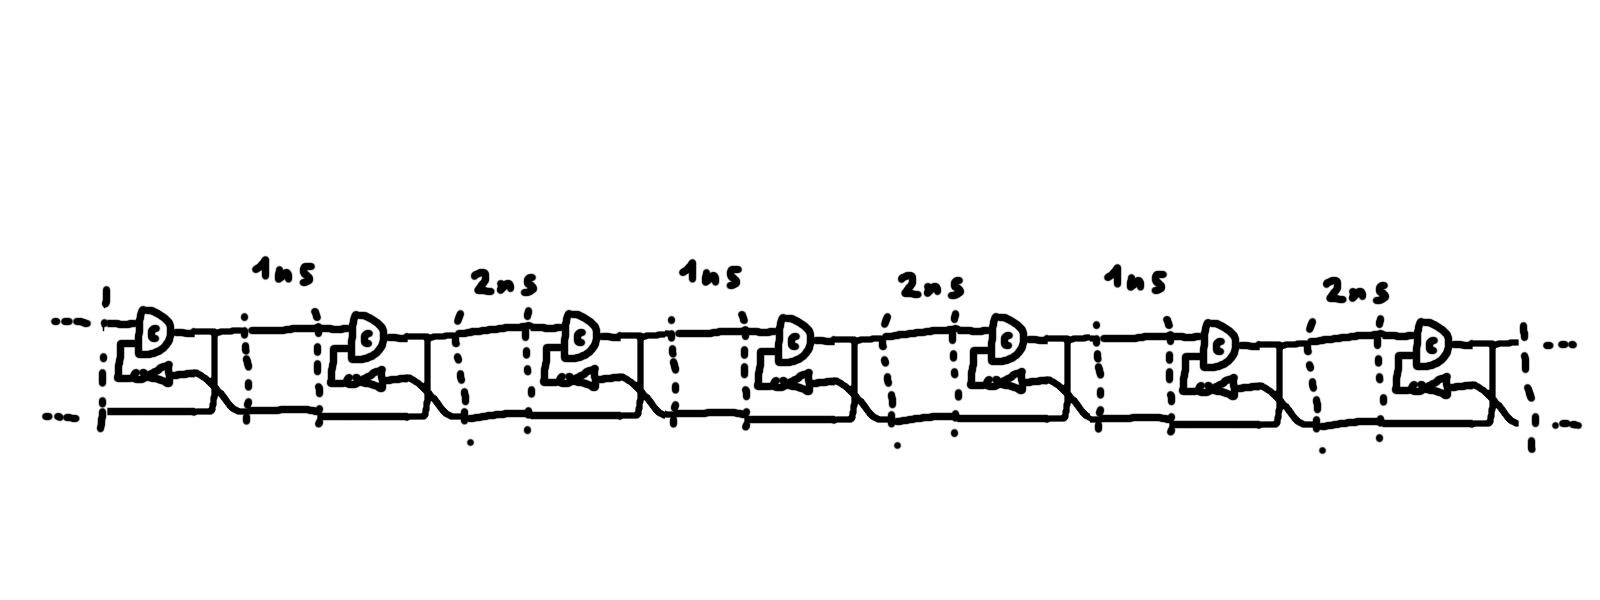
\includegraphics[width=0.7\linewidth]{slike/dly5}
	\caption{}
	\label{fig:celement}
\end{figure}


\section{Teoretične osnove} \label{a}
Poglejmo si sedaj teoretične osnove asinhronih vezji. Naredili bomo kriterijje, katerim naše vezje mora slediti, da bo delovalo zanesljivo.



\subsection{Indikacija} \label{b}

Indikacija je pomemeben koncept pri asinhronih vezjih. Signal je indiciran, če ima vsaka njegova sprememba posledice. Prestaavljajmo si ALI logična vrata. Recimo, da je stanje na vhodu 0,0. Če en signal preklopi, se spremeni stanje izhoda, torej ima sprememba posledice. Če sedaj preklopi še drugi signal, se stanje na izhodu ne spremeni. To pomeni, da ne vemo če se je drugi signal že spropagiral od vira. Po drugi strani, če originalni signal preklopi nazaj, se izhod ponovno spremeni. Če ne želimo uporabljati časovnih predpostavk, mora vsak preklop vsakega signala biti indiciran. To pomeni, da mora na vhodu ALI in IN vrat signal vedno preklopiti dvakrat zaporedno, na vhodu C elementa morata signala preklopiti eden za drugim itd. 

\subsection{Hitrostna neodvisnost} \label{b}

Naredimo model asinhronih vezji, da bolje razumemo kako delujejo. Predstavljajmo si vezje vrat, povezanih med seboj. Vsaka vrata imajo vhodne in izhodne signale. Ko vhod vrat diktira spremembo izhoda postanejo vrata aktivna. Po neznanem časovnem zamiku se spremeni tudi izhod. Zanimivo je, kar se zgodi na izhodu vrat. Vrata ki imajo na vhodu izhodini signal naše originalnih vrat imajo tri opcije.
Lahko sprememba vhoda ne spremeni izhoda.
Lahko sprememba vhoda ne povzroči spremembe izhoda.
Lahko pa so bila vrata aktivna, a zaradi spremembe izhoda sedaj niso več aktivna.

Asinhrona vezja delujejo pravilno, če se zadnji kriterij nikoli ne zgodi.

Obstajajo različni razredi asinhronih vezji, kjer je ta kriterij realiziran z različnimi predpostavkami.

\subsection{Hitrostna neodvisnost} \label{b}
Hitrostno neodvisna vezja imajo neznane zakasnitve v vratih in nimajo zakasnitev v žicah. To žal ni zelo realno v današnjih vezjih, kjer so zakasnitve v žicah lahko velik del zakasnive v logičnih vejah. Še posebaj pa to ne velja v FPGA, zato ta vezja niso zelo zanesljiva.

\subsection{Zakasnilna neodvisnost} \label{b}

Vezja, ki so neodvisna na zakasnitve imajo neznane zakasnitve v žicah in vratih, tu ne predpostavimo nič, ampak S takimi vezji ne moremo procesirati podatkov. Citat

\subsection{Kvazi-zakasnilna neodvisnost} \label{b}
Srednja pot je kvazi zakasnitvena neodvisnost, kjer imamo določene predpostavke, o zakasnitvah v le določenih žicah.

